\subsection{風景生成部}
風景生成部はデータ取得部で取得したStreetViewの情報からパノラマ画像の生成,道路部分切り抜きを行い,出力部へと送る風景画像を生成する処理群である.
\subsubsection{パノラマ画像生成}
パノラマ画像の生成にはGSVPanoライブラリを利用した\cite{GSVpano}.GSVPanoライブラリはGoogleStreetView からパノラマ画像を作成するライブラリである.パノラマ画像の生成は図\ref{figure:panorama}のようにパノラマ表示されたGoogleStreetViewについて複数の視線の向きで28枚の画像を取得する.その後パノラマ画像になった時,隣接する部分の画像どうしを結合することで一枚のパノラマ画像を生成する.
その後システムは生成したパノラマ画像トリミングすることで余白部分の削除を行う.

\begin{figure*}[ht]
\begin{center}
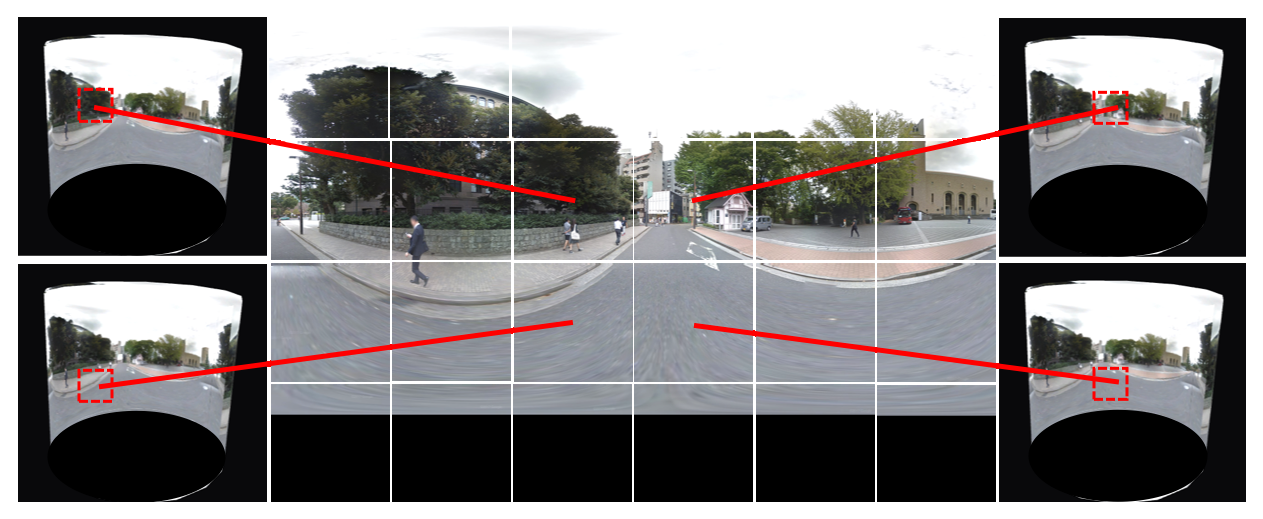
\includegraphics[width=17cm]{img/04_detail/make_panorama.eps}
\end{center}
\caption{パノラマ画像の生成}
\label{figure:panorama}
\end{figure*} 

\clearpage

\subsubsection{道路部分切り抜き}
StreetView 取得部で取得した画像に対し道路部の切り抜きを行う. 切り抜きにはマスク処理を用いる. マスク画像は事前に手動で StreetView の道路部分を黒くし, 風景部分を白くすることで作成した. StreetView取得部で取得した画像に対し図\ref{figure:trim}のようにマスク画像を用いてマスク処理を行い道路部分を切り抜く.


\begin{figure}[h]
\begin{center}
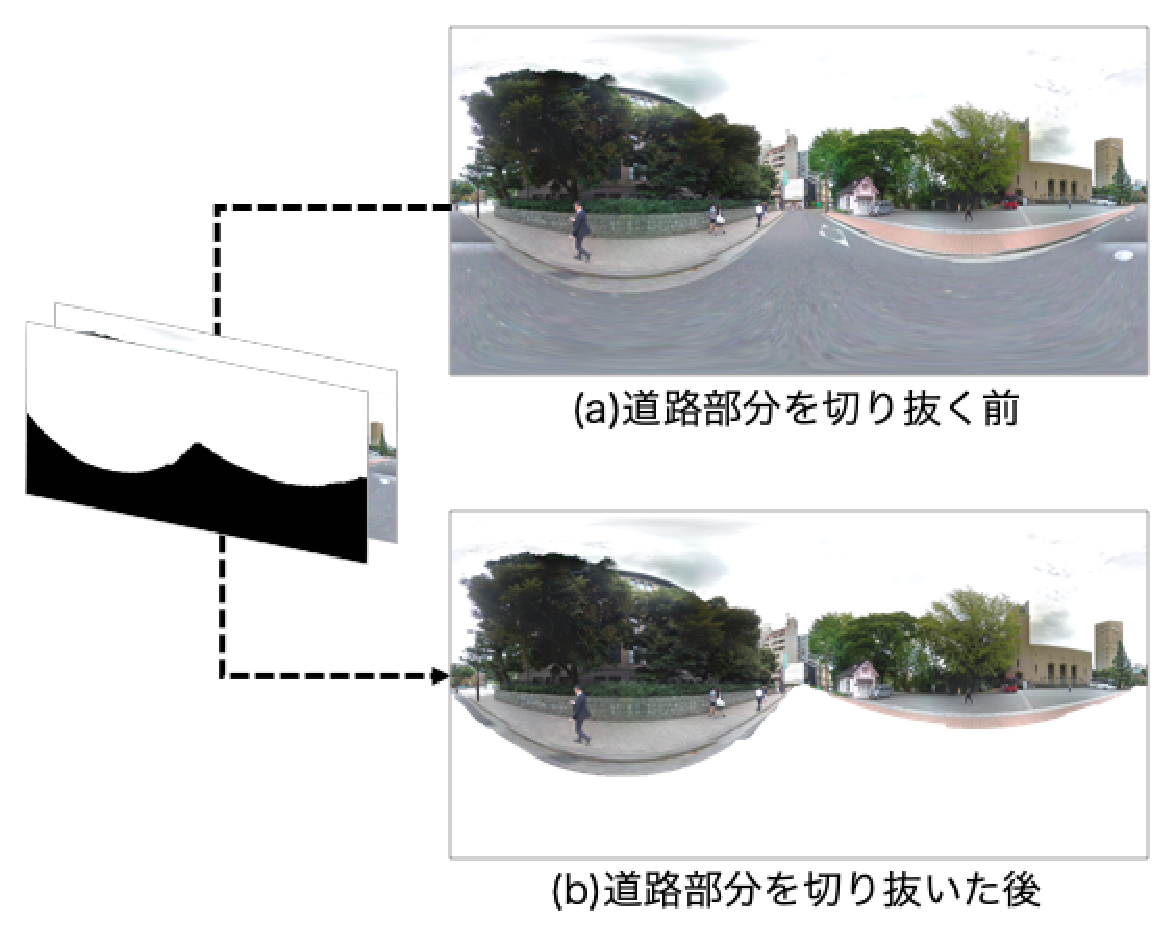
\includegraphics[width=11cm]{img/04_detail/triming.eps} 
\end{center}
\caption{マスク処理による道路部分の切り取り}
\label{figure:trim}
\end{figure} 